\chapter{Description Les interfaces de Réalisation }


\section*{introduction}

Nous allons introduire dans ce chapitre les interfaces graphiques que nous avons dû
à réaliser, nous vous présentons ces interfaces sous formes captures d'écran, ainsi que des
explications montrant le déroulement de notre application :




\section{Connection:}
Pour accéder à notre application l'utilisateur doit se connecter ou creér un compte . Comme toutes les applications qui comportent des informations personelles, la sécurité d'accès est nécessaire. La figure ci-après donne l'interface à travers laquelle l'utilisateur s'identifie. Il saisit son E-mail et son mot de passe puis l'application  vérifie si cet utilisateur existe en base donnée ou pas.

\begin{figure}[H]
  \centering
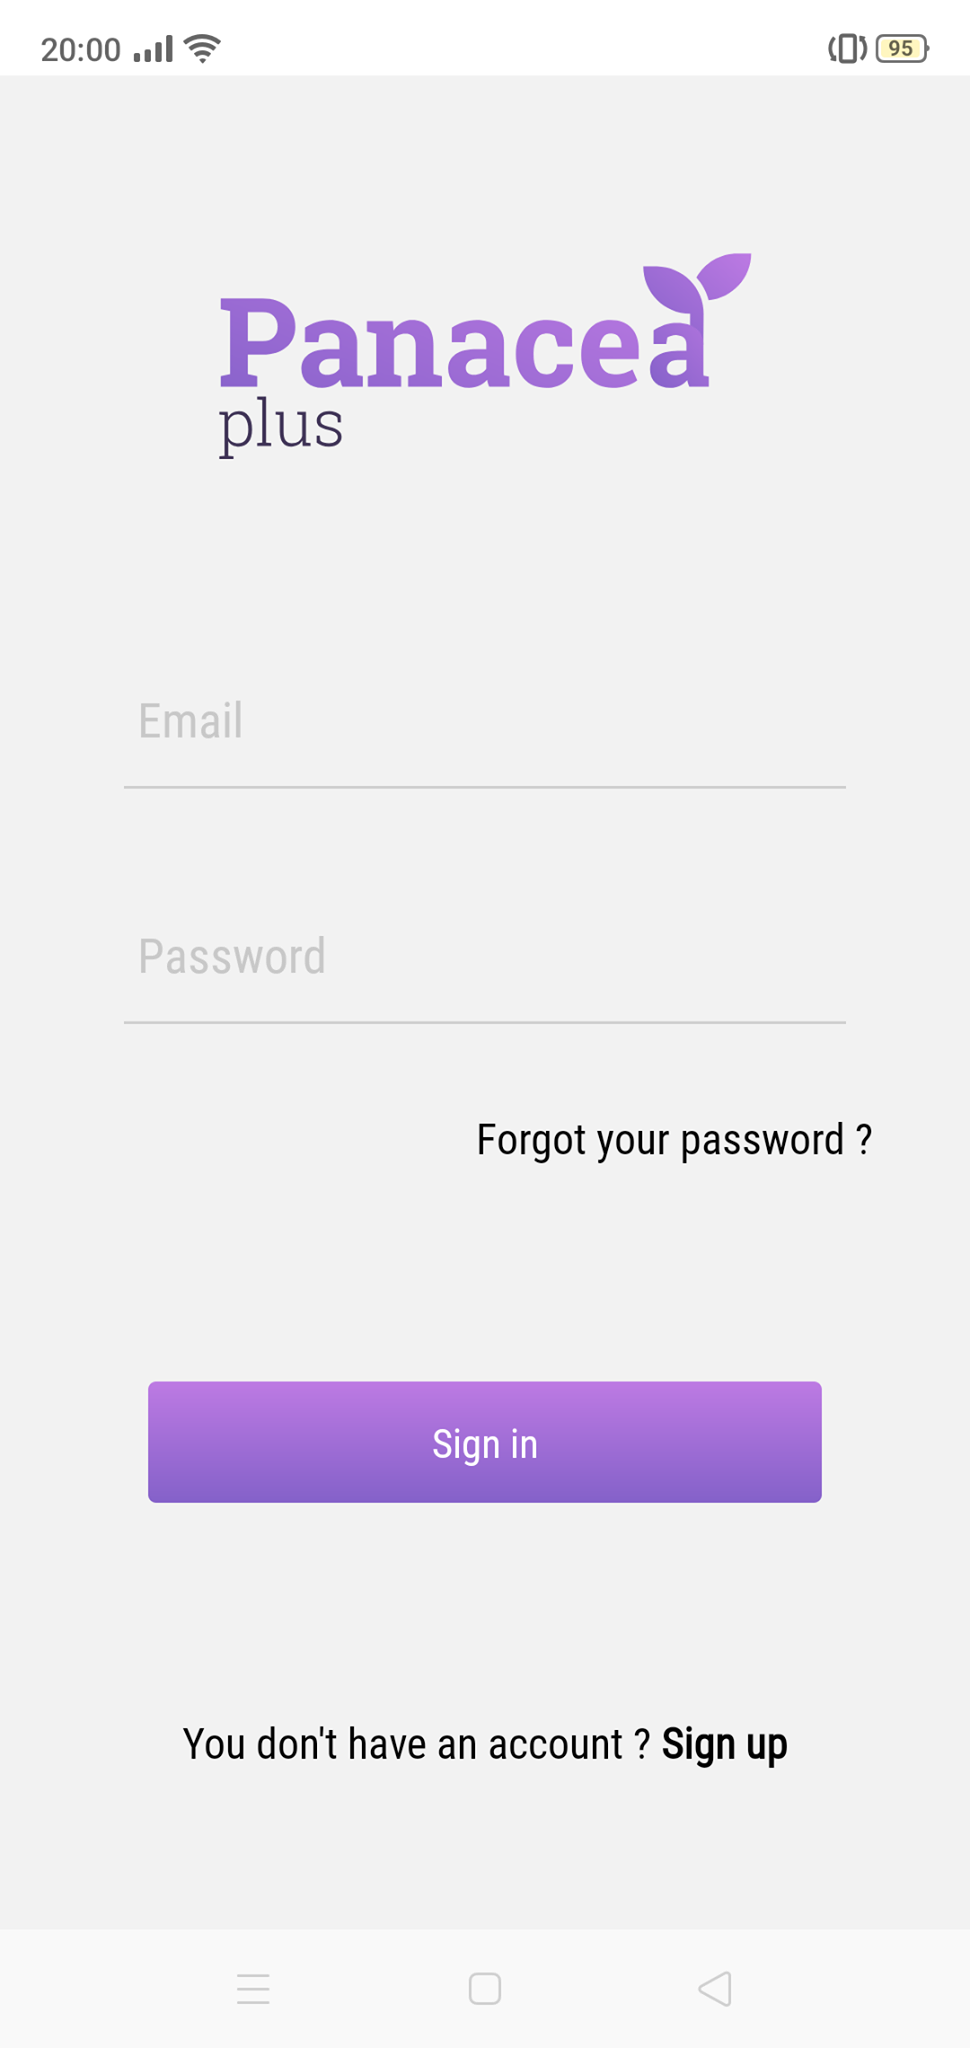
\includegraphics[width=11cm,height=11cm,keepaspectratio]{Application/connecter.png} 
\caption{Interface de se connecter}
\end{figure}

Le message d'erreur sera afficher dans le cas où les information n'existent pas dans notre base de données ou dans le cas d'abscense d'accès à l'internet.
\begin{figure}[H]
  \centering
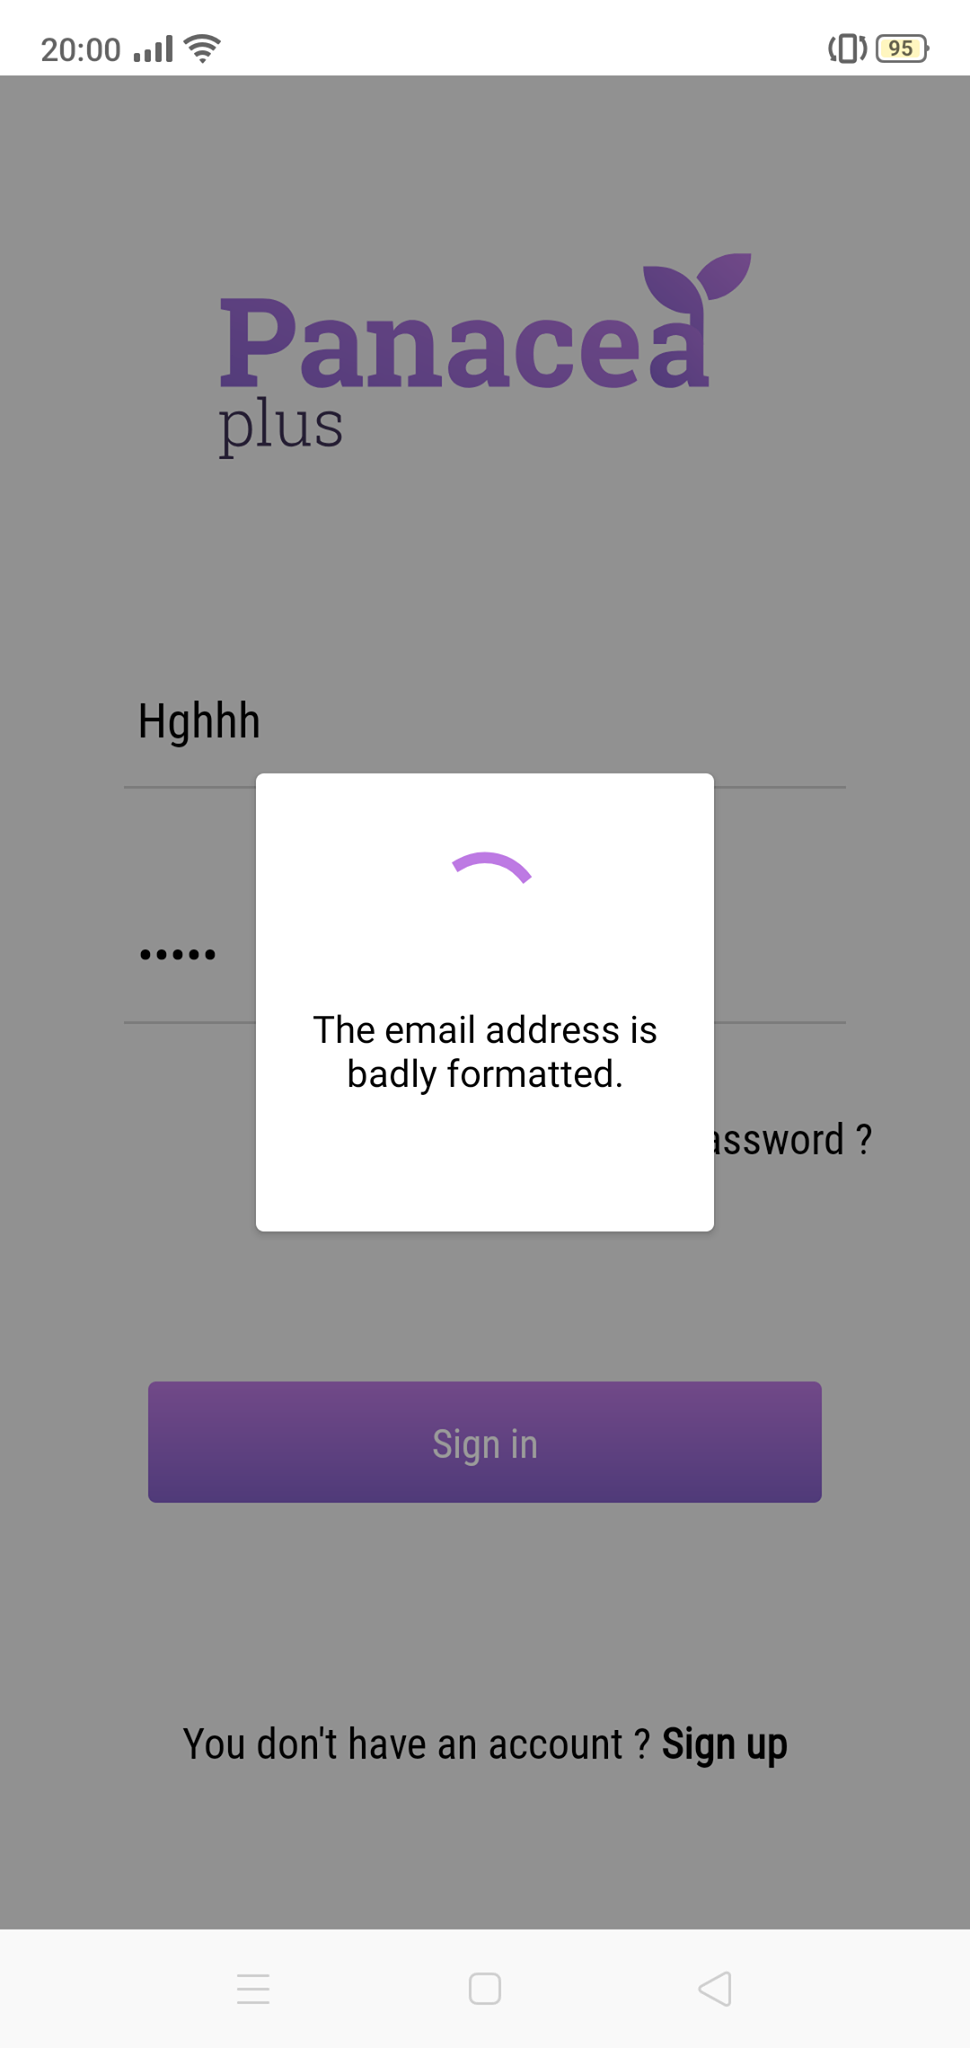
\includegraphics[width=8cm,height=8cm,keepaspectratio]{Application/er.png} 
\caption{Interface de connection en cas d’erreur}
\end{figure}

Une fois les données sont valides, l'utilisateur peut accéder à la page d'accueil.
% Les utilisateurs principaux de l'application sont les médecins et les patients , chaque utilisateur a sa propre interface d'accueil.
\section{Inscription}

Pour créer un nouveau compte il faut d'abord que l’utilisateur  appuie sur Sing up (première interface ) après l'application il va dirige l'utilisateur vers l'interface de l'inscription
% choisie s'il est un médecin ou un patient puis il va être diriger vers l'interface suivant pour saisie ses informations :
% \begin{figure}[H]
%   \centering
%   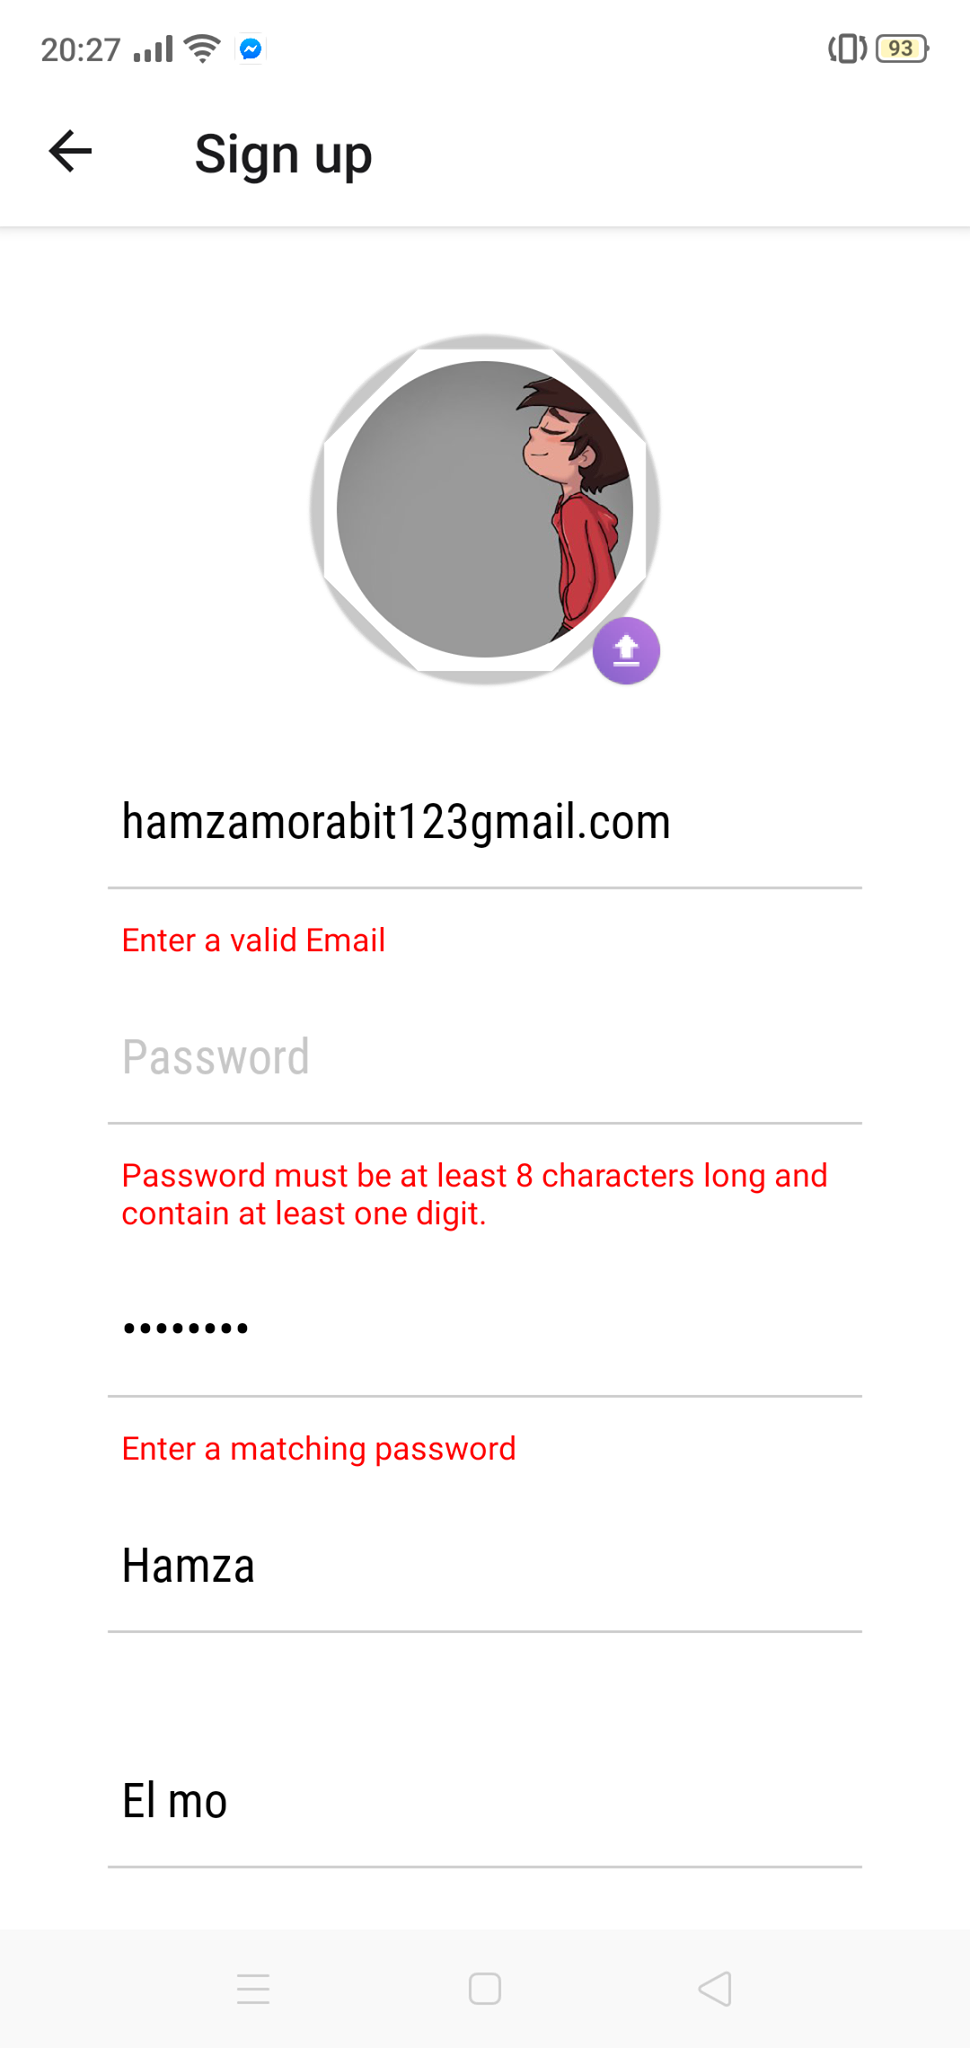
\includegraphics[width=7cm,height=7cm,keepaspectratio]{Application/insc1.png} 
% \caption{Interface d'inscription pour choisir type d'utilisteur}
% \end{figure}
\begin{figure}[H]
  \centering
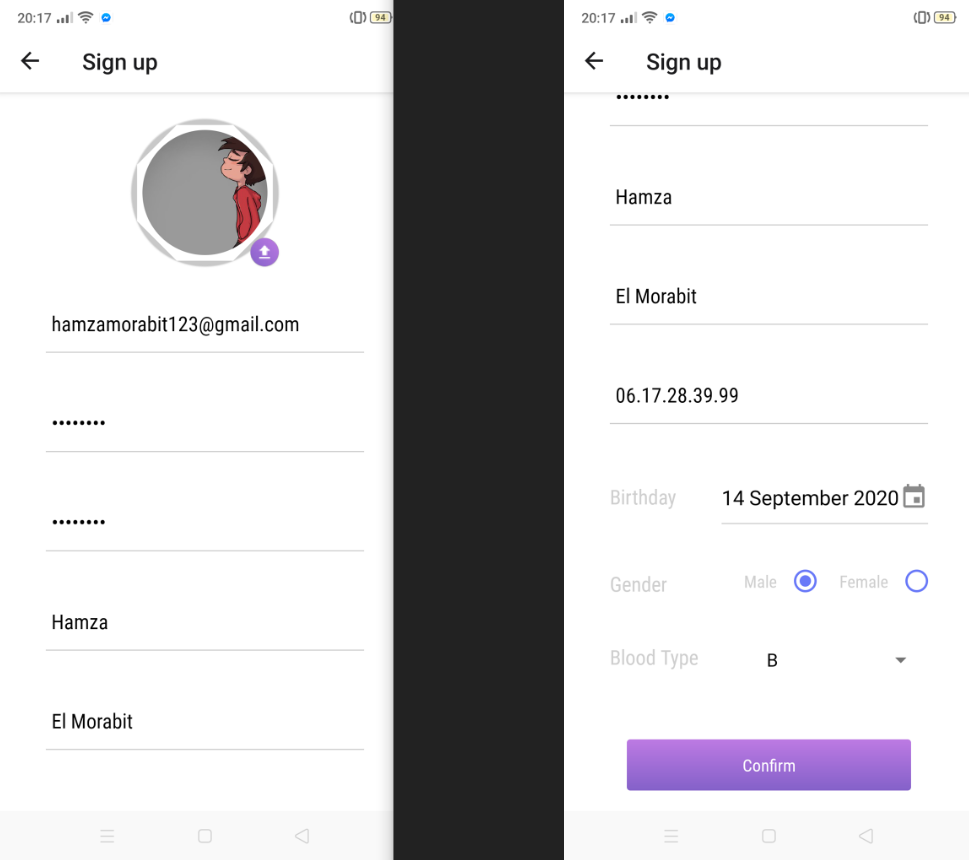
\includegraphics[width=10cm,height=8cm,keepaspectratio]{Application/med1.png} 
\caption{Interface de saisie les informations d'un nouveau compte}
\end{figure}


puis , il faut remplir tous les champs pour créer un nouveau compte sinon un message d'erreur s'affichera à l'interface comme on voit au-dessous .
\begin{figure}[H]
  \centering
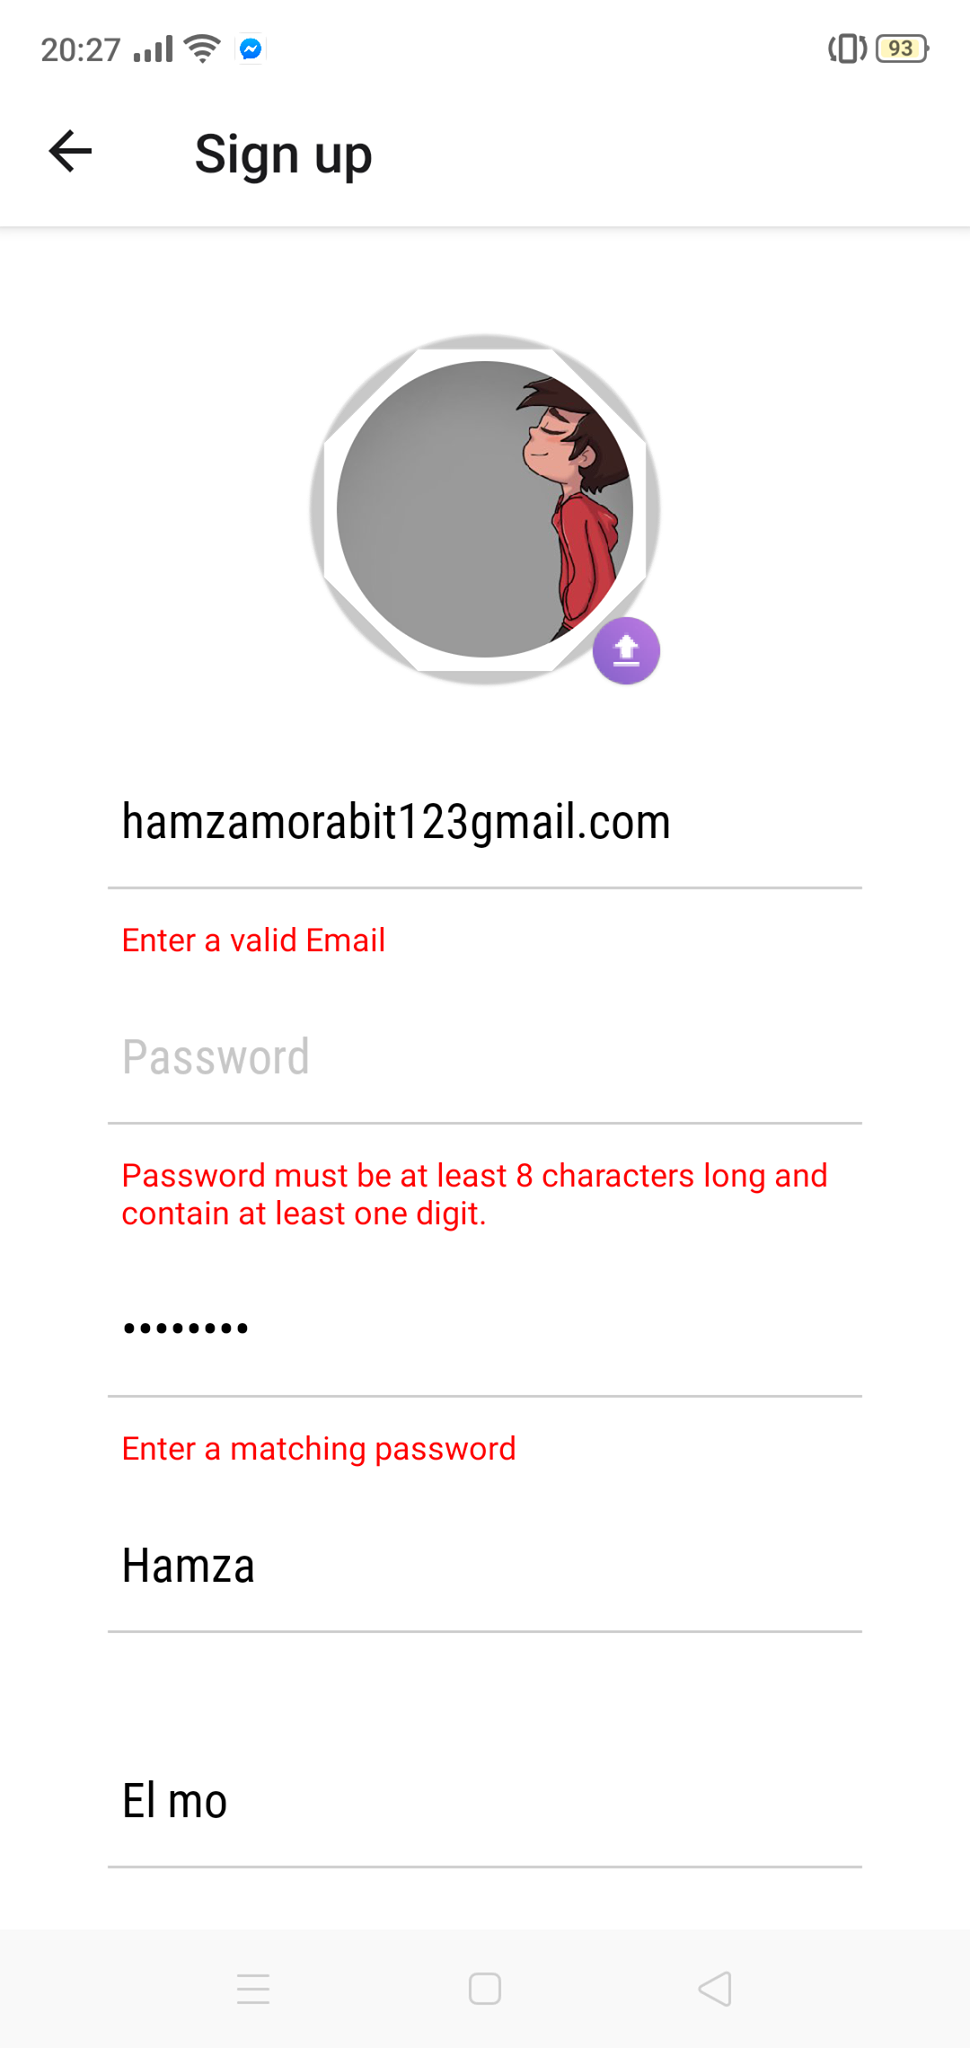
\includegraphics[width=8cm,height=8cm,keepaspectratio]{Application/insc1.png} 
\caption{Interface de saisie les informations d'un nouveau compte en cas d'erreur}
\end{figure}




\section{Consulter la profile }
\begin{figure}[H]
  \centering
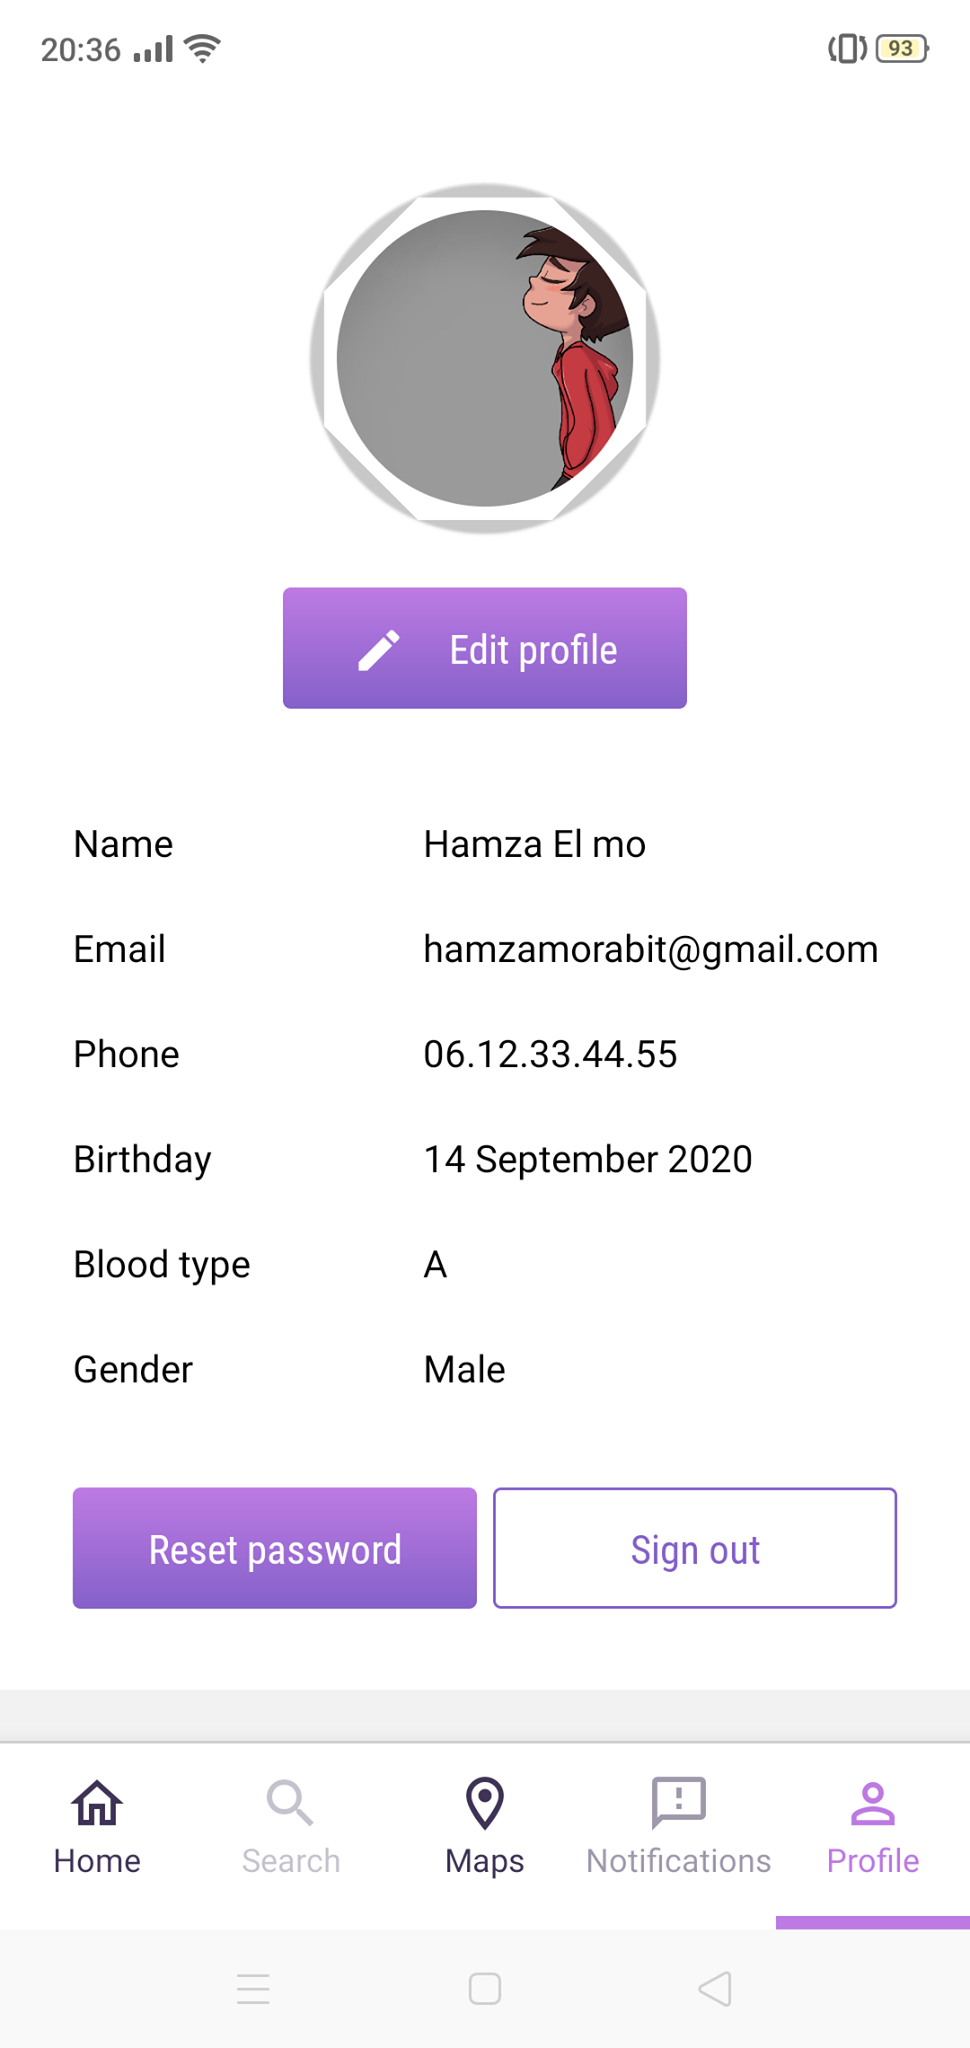
\includegraphics[width=10cm,height=8cm,keepaspectratio]{Application/med22.png} 
\caption{Interface de  consulter le profil}
\end{figure}


Cette interface contient des champs textes dans lesquels il y'a les informations que l'utilisateur a déja insérer en création du compte.
Les champs ne sont pas éditables, on ne peut pas les modifier seulement si on clique sur la boutton 'Edit profil', dans ce cas là les champs deviennent éditables ( indiqué ci-dessous ).
Tous les modifications seront modifier aussi à la base de données.
\begin{figure}[H]
  \centering
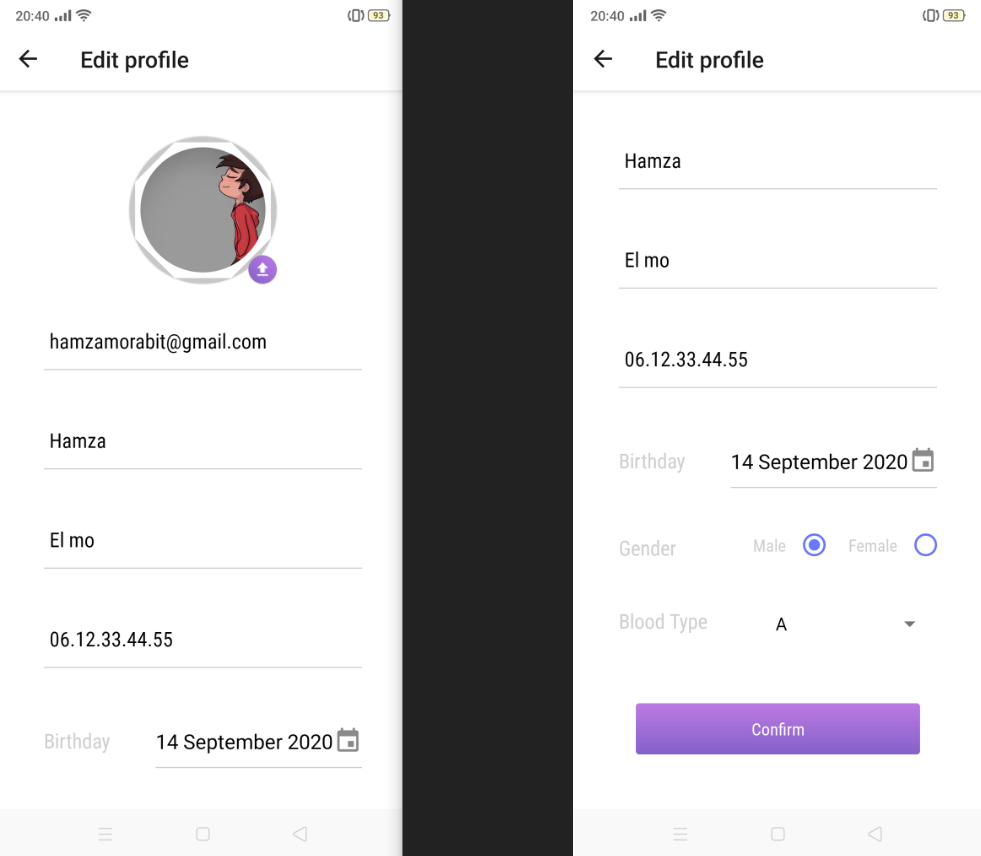
\includegraphics[width=10cm,height=8cm,keepaspectratio]{Application/medd.png} 
\caption{Interface de modifier le profil}
\end{figure}

\section*{Page d’accueil }
\begin{figure}[H]
  \centering
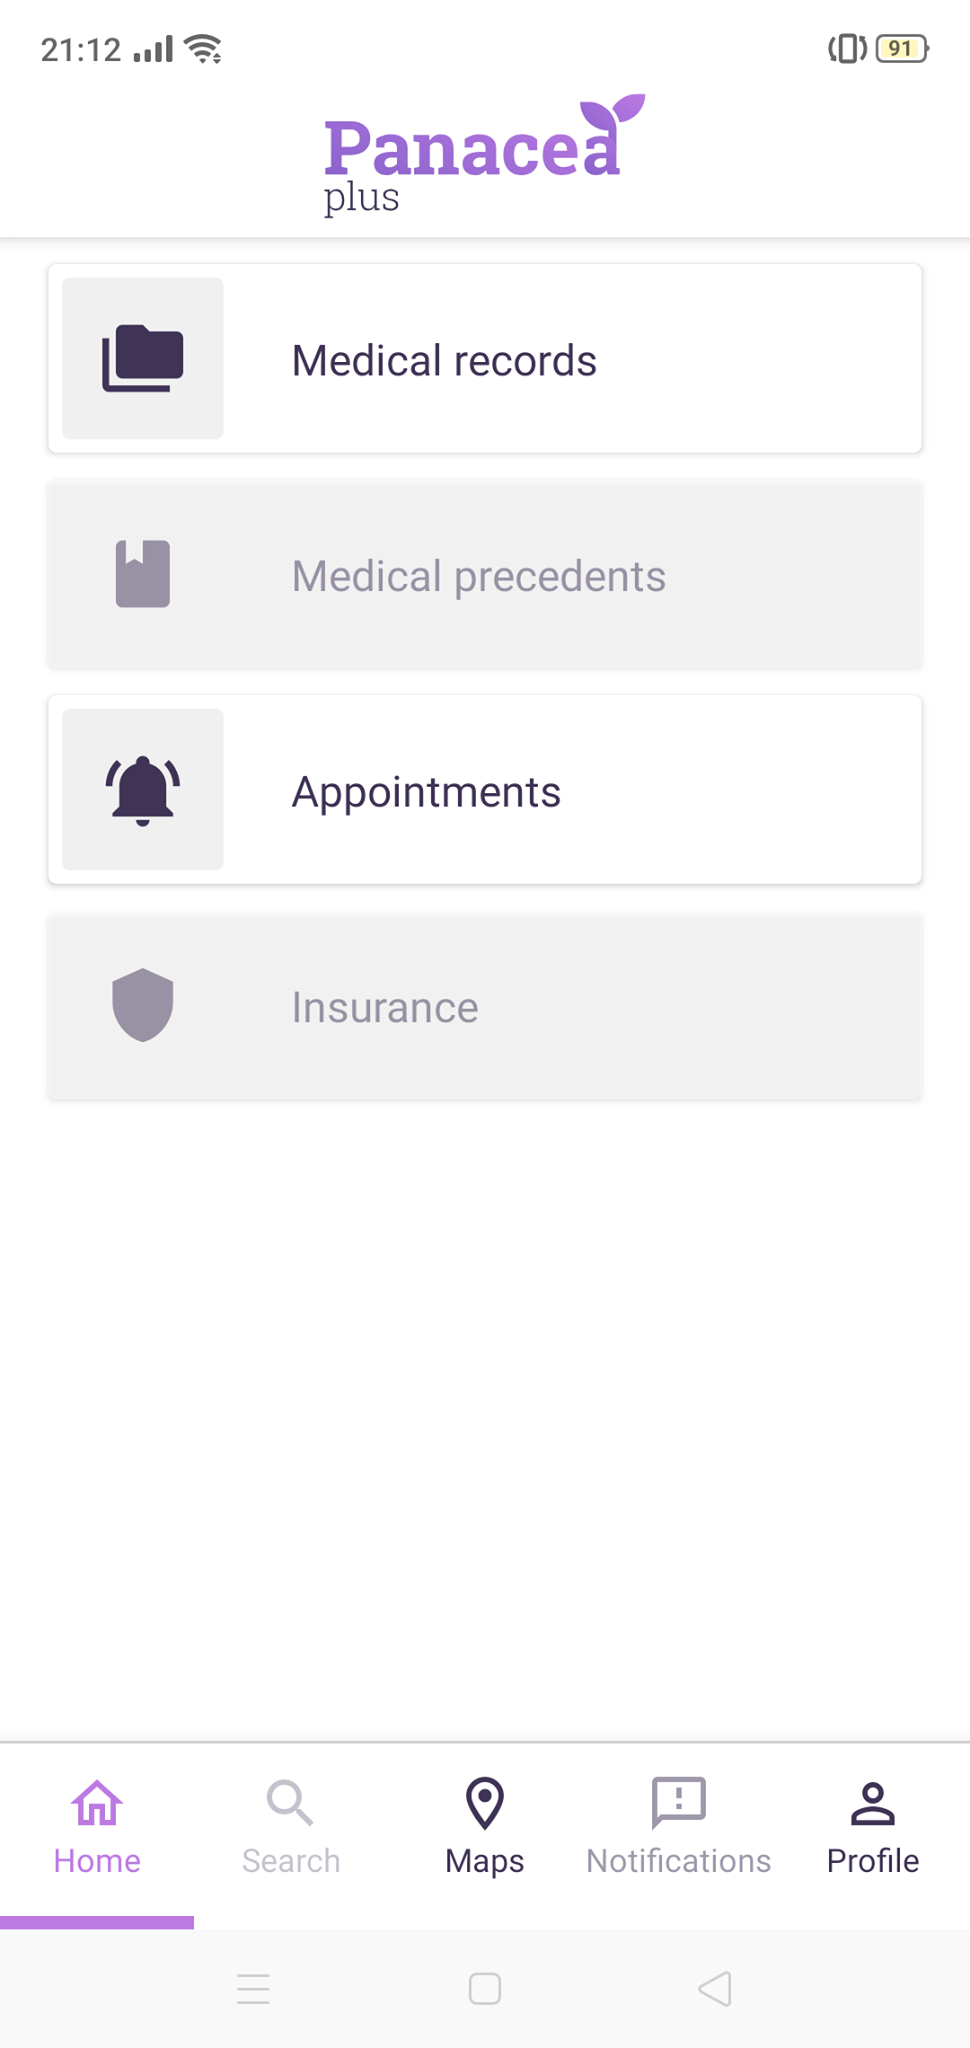
\includegraphics[width=9cm,height=7cm,keepaspectratio]{Application/acc.png} 
\caption{Menu de l'application}
\end{figure}



% \section{Des interfaces du patient }
\subsection{Réinitialiser Mot de Passe }
La figure ci-dessus montre la page d’accueil qui va apparaitre dès que l'utilisateur appuie sur 'resetPassword'  . Cette interface  à un rôle très un important parfois l'utilisateur à oublier son code l'utilisateur il a cette  solution pour récupérer leur code car celle-ci fonctionnera d'une façon sécurisée 
\begin{figure}[H]
  \centering
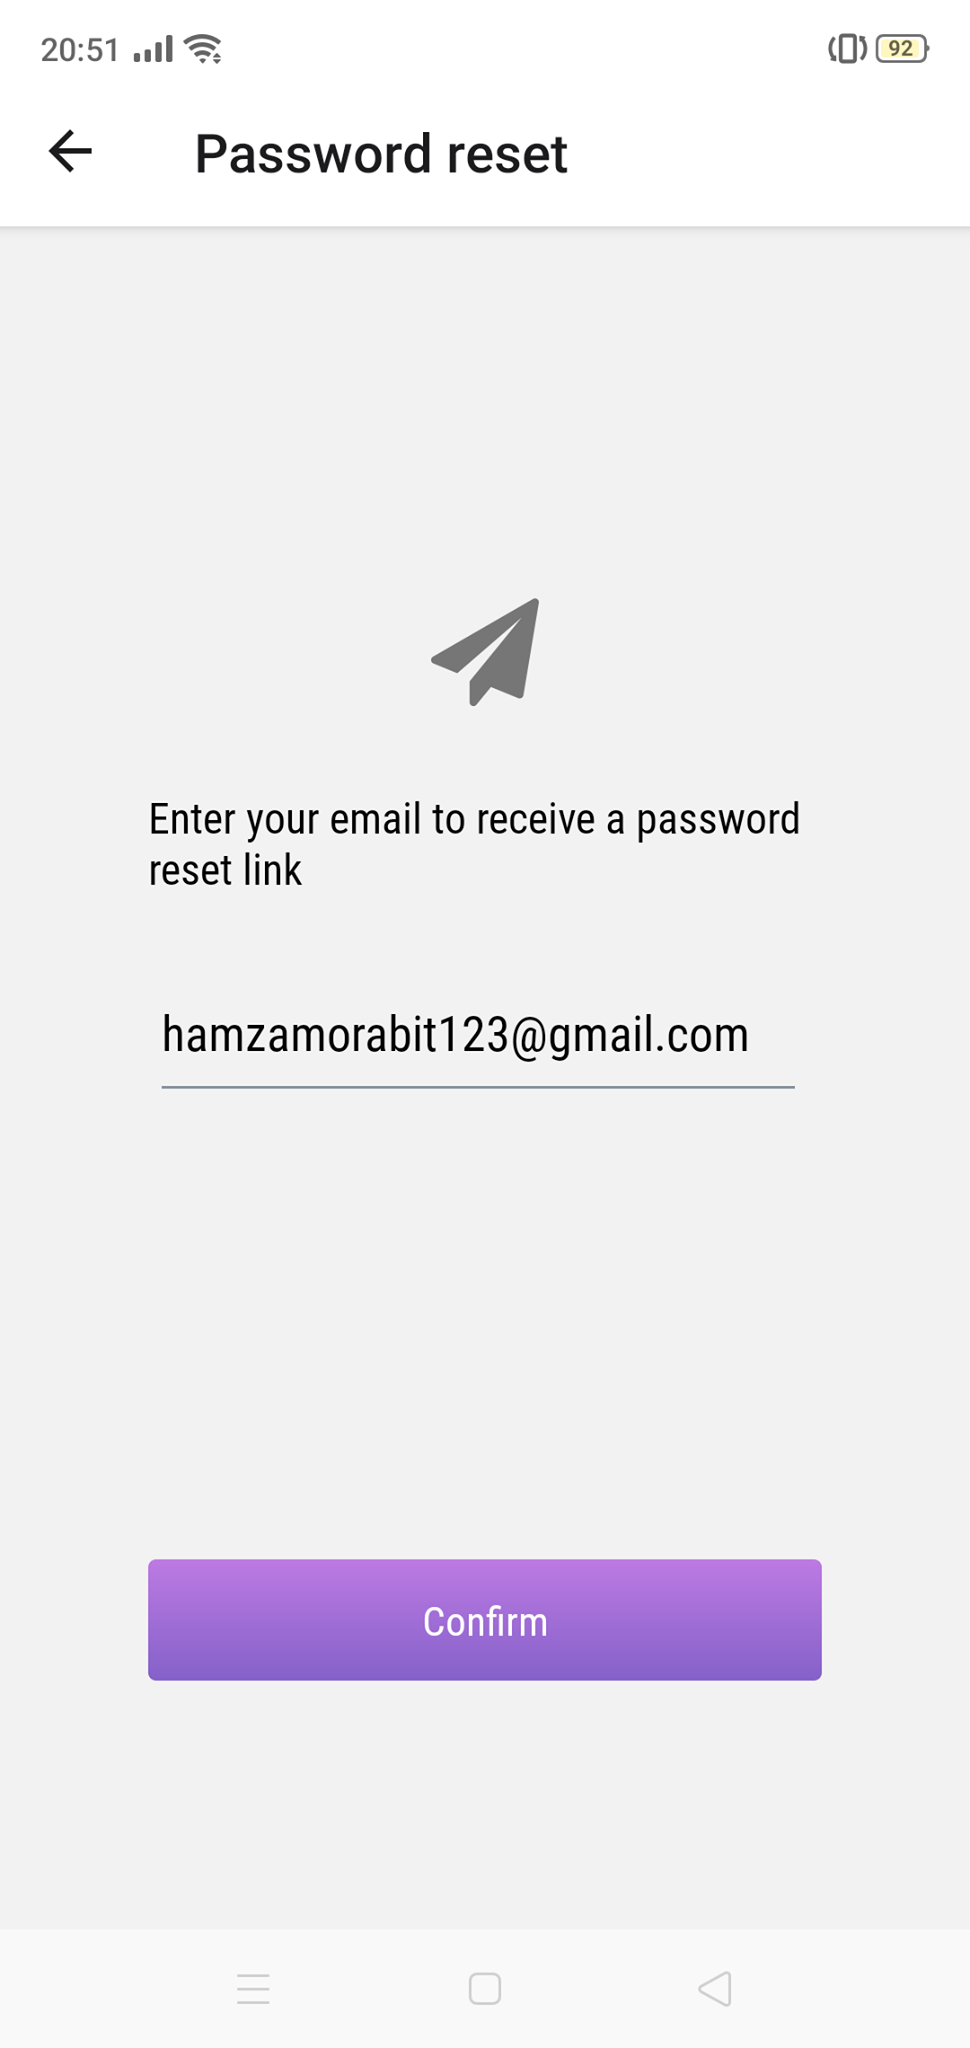
\includegraphics[width=9cm,height=7cm,keepaspectratio]{Application/err2.png}
\caption{Interface de réinitialiser Mot de Passe}
\end{figure}
Si L'utilisateur a saisi un mail qui ni correct ni dans la base de données l'interface dirige l'utilisateur sur une autre   interface (ci-dessous)
\begin{figure}[H]
  \centering
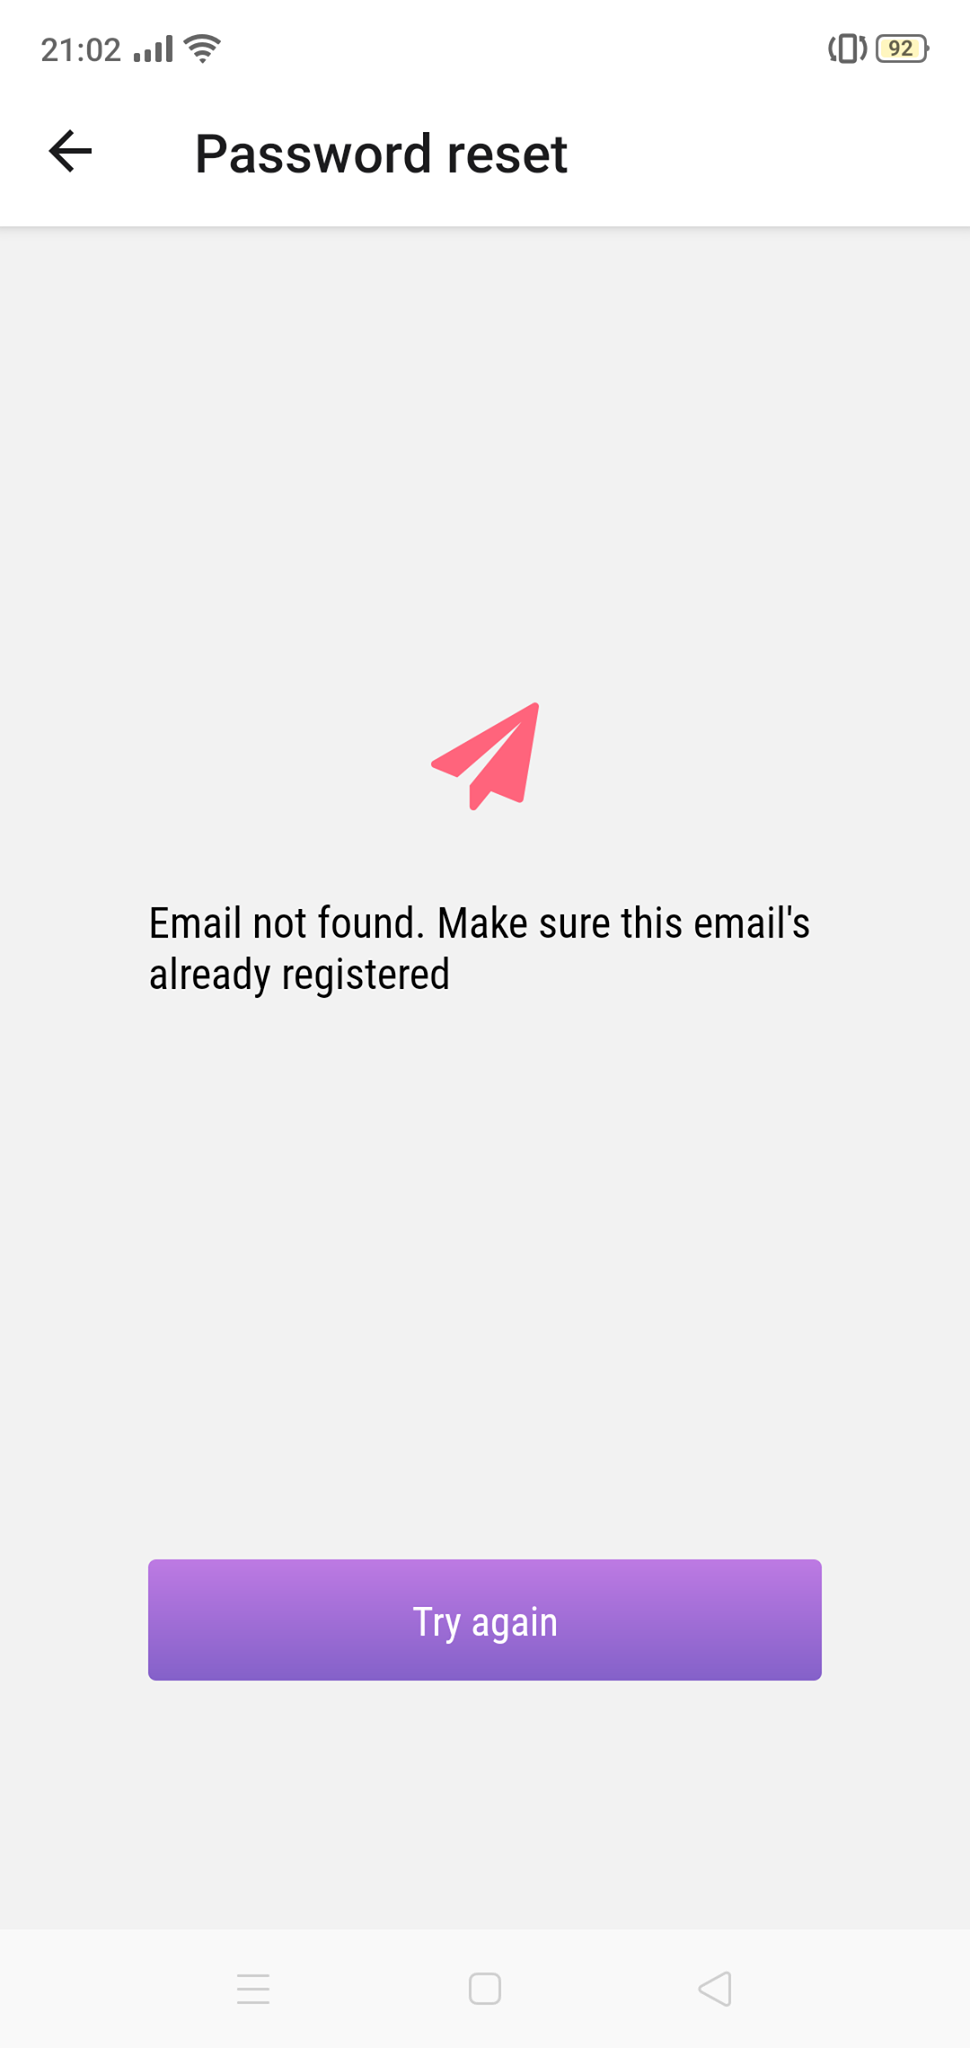
\includegraphics[width=9cm,height=7cm,keepaspectratio]{Application/ert.png}
\caption{Interface de réinitialiser Mot de Passe en cas d'erreur}
\end{figure}



\subsection{Rendez-vous}
Permet de programmer les rendez-vous et comprend aussi bien :\\
* programmation des visits à effectué aux docteurs .\\
* Remarque des docteurs ( orodonnace pharmacetique , d'analyse ..)\\
* La date 
\begin{figure}[H]
  \centering
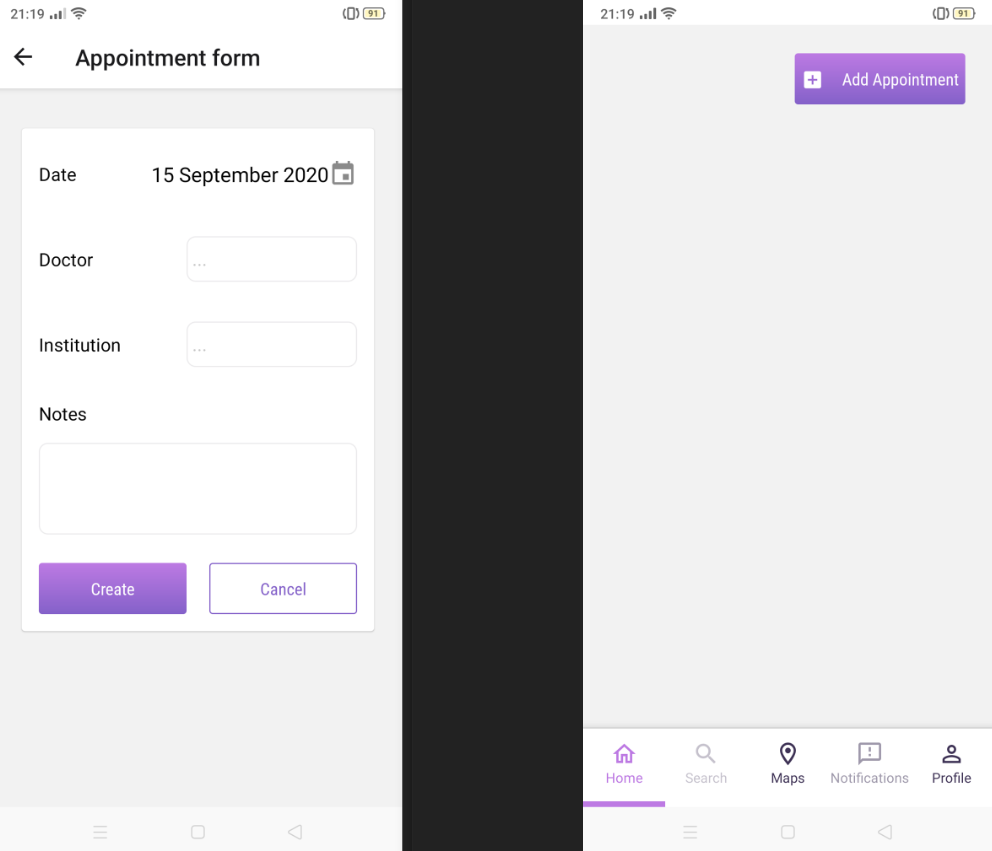
\includegraphics[width=9cm,height=7cm,keepaspectratio]{Application/app0.png} 
\caption{Interface de prendre un rendez-vous}
\end{figure}
L'application permet aussi à l'utilisateur de modifier ou supprimer certain rendez-vous
\subsection{Recherche l’emplacement}
La carte (Maps) permet de choisir et localiser les cabinets les plus proches et faciliter l'accessibilité

\begin{figure}[H]
  \centering
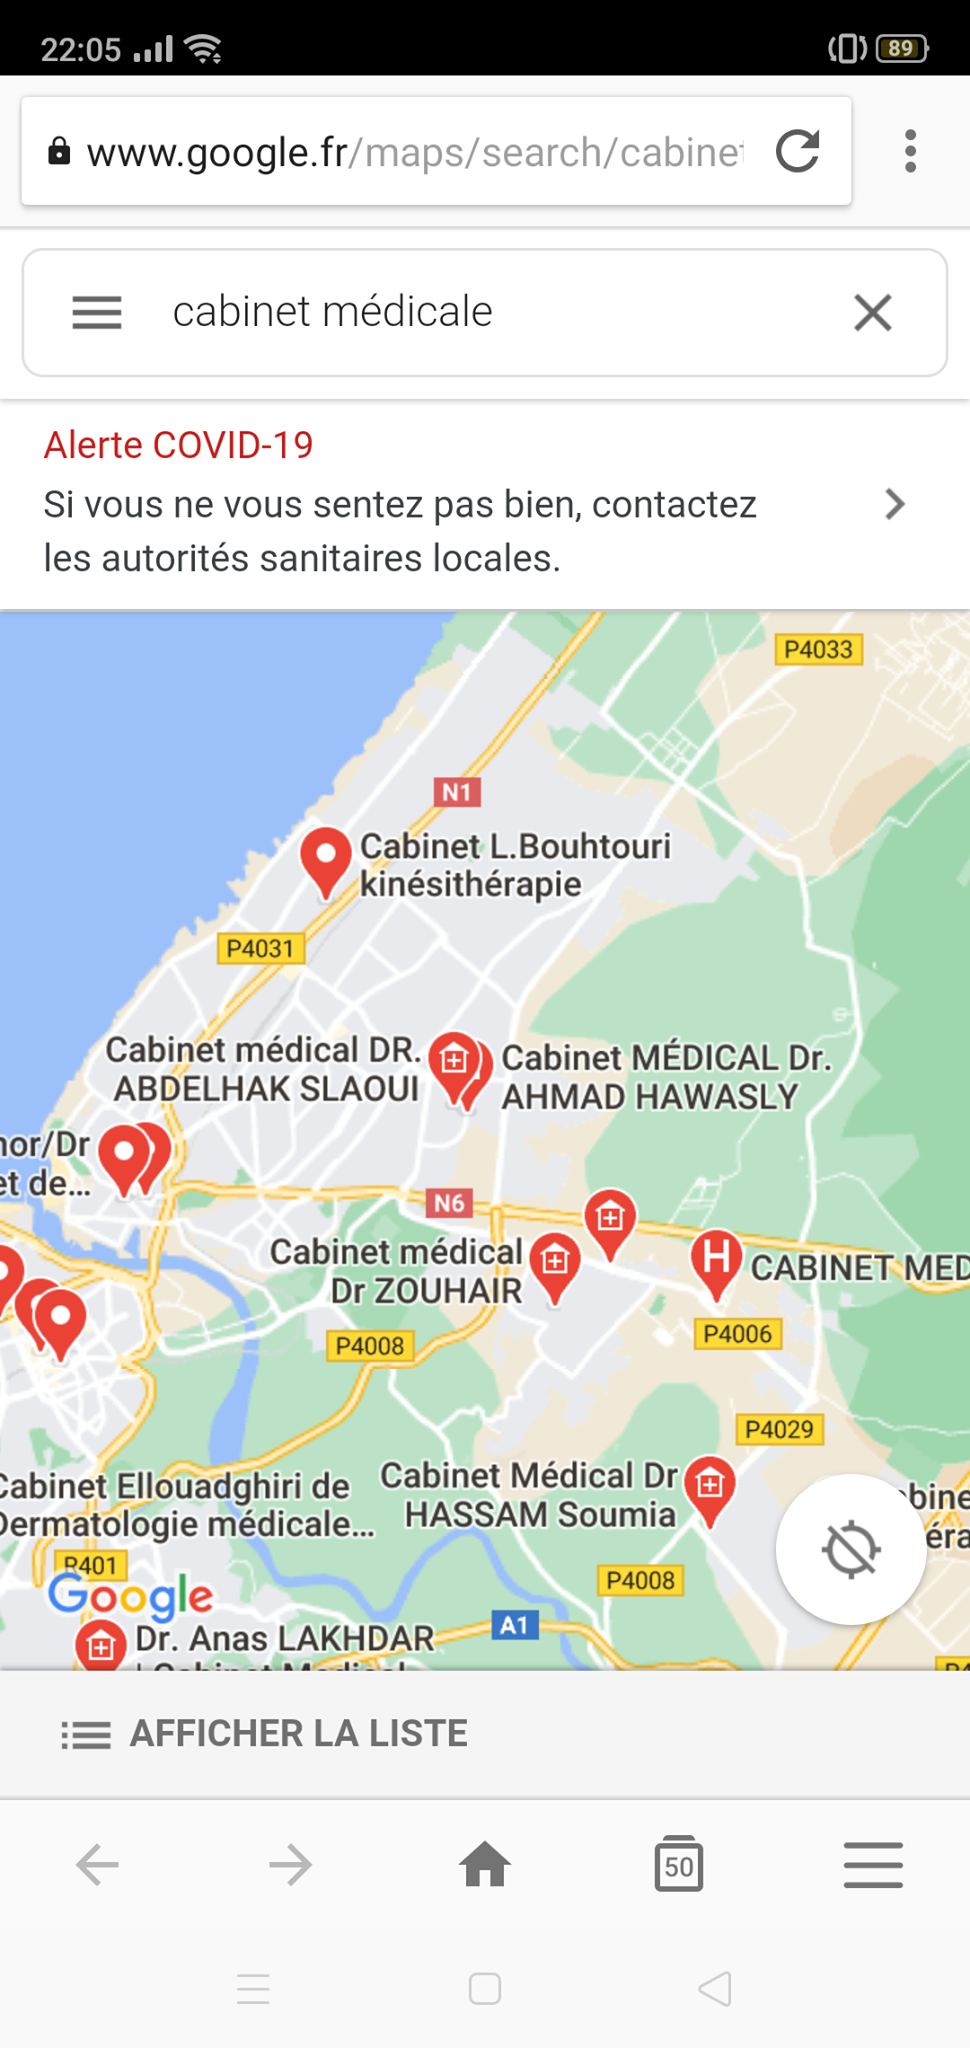
\includegraphics[width=9cm,height=8cm,keepaspectratio]{Application/map.png} 
\caption{Indiqué les  cabinets les plus proche}
\end{figure}
pour accéder à cette carte il faut d'abord avoir l'accord à sa demande

\begin{figure}[H]
  \centering
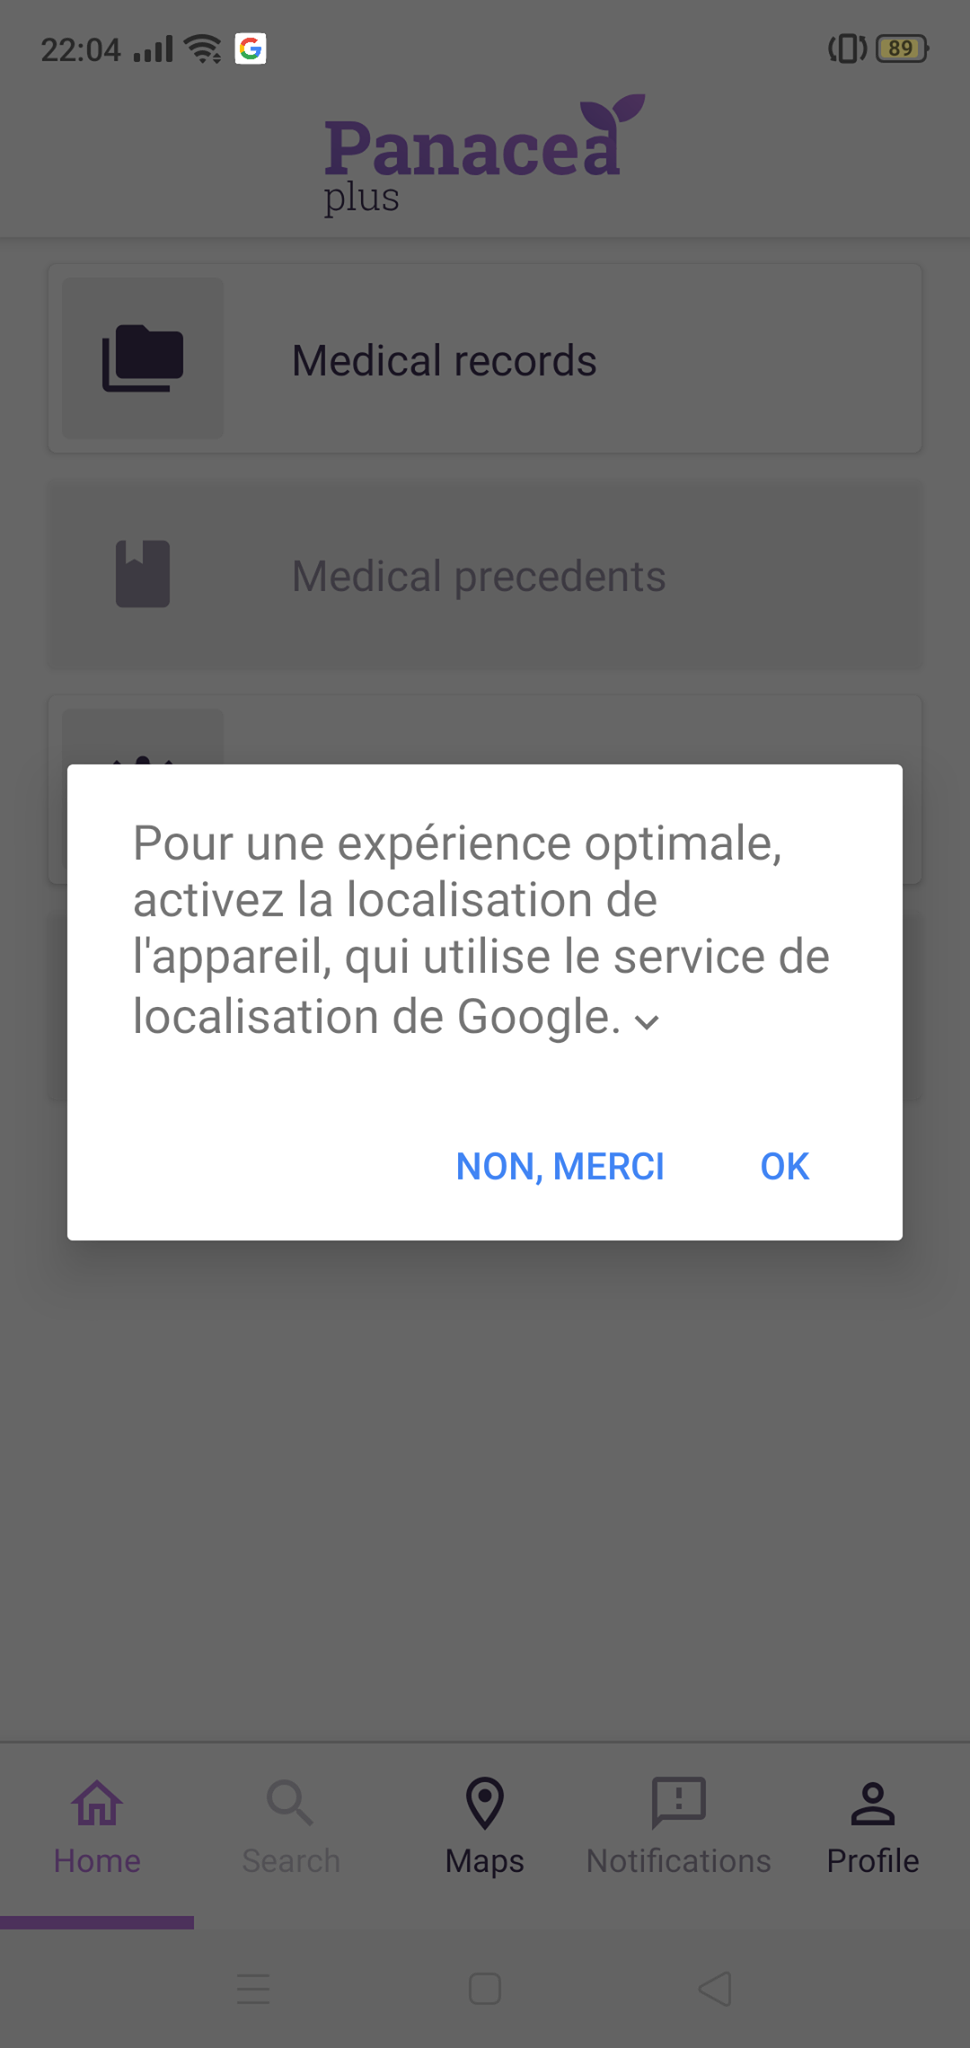
\includegraphics[width=9cm,height=8cm,keepaspectratio]{Application/auto.png} 
\caption{Interface affichage d'un messge d'accessibilité}
\end{figure}
 \subsection{Rapports médicaux }

  \subsubsection{problème cardiaque}
  Cette interface me permet d'enregistrer et de modifier  le rapport et le bilan cardiaque du docteur
  \begin{figure}[H]
  \centering
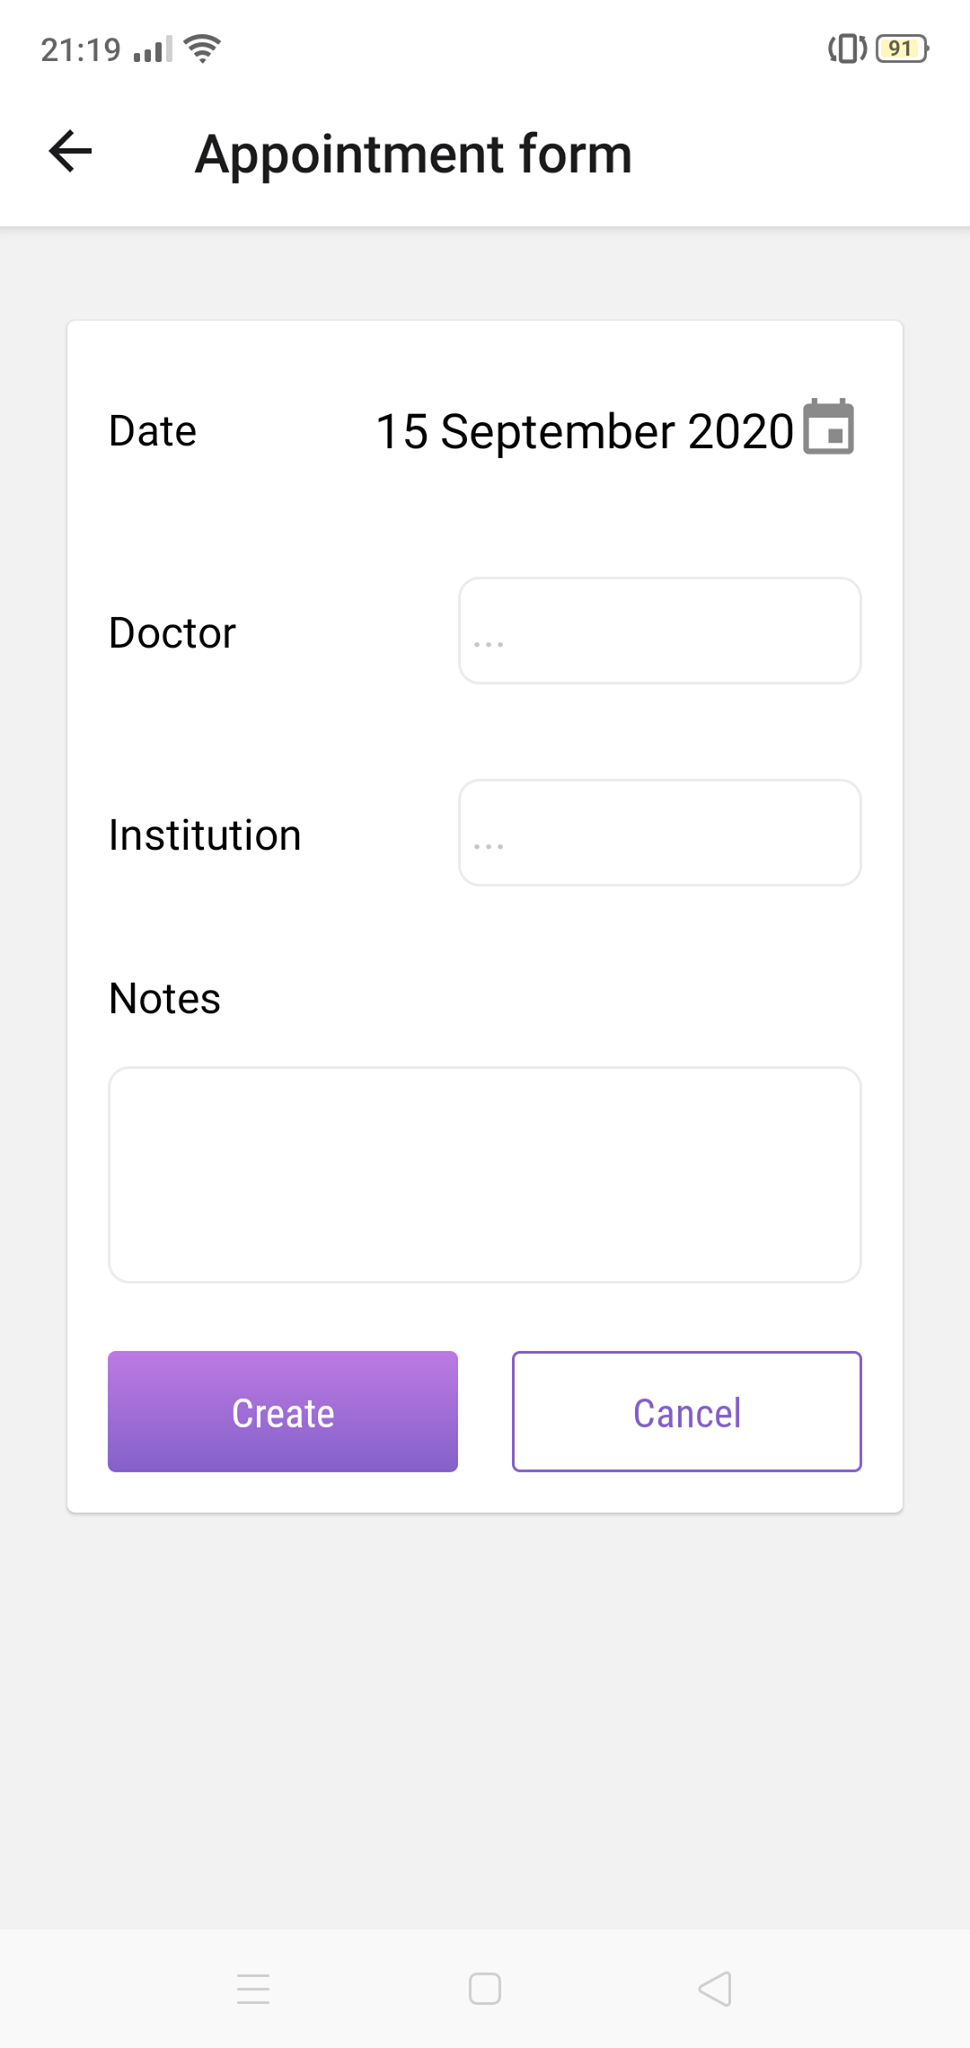
\includegraphics[width=9cm,height=8cm,keepaspectratio]{Application/bil.png} 
\caption{Interface affichage d'un messge d'accessibilité }
\end{figure}
% % cette fragement contient les informations personelle du patient et les valeurs du paramètres vitaux (Taille,Poids,Temperature,Pouls,Respiration,Glycemie capillaire,Tension et groupe sanguin).
% \subsection*{Diagnostic:}
% \begin{figure}[H]
%   \centering
% 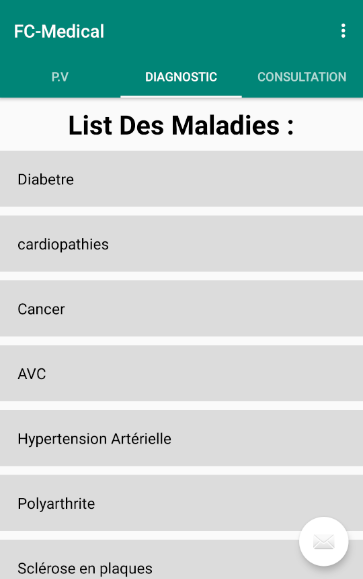
\includegraphics[width=7cm,height=7cm,keepaspectratio]{Application/dossier3.png} 
% \caption{ Interface de Diagnostic}
% \end{figure}

% Contient diagnostic de ces maladies suivants (Diabète, cardiopathies, cancer, AVC, hypertension artérielle, polyarthrite, sclérose en plaques, maladie de Crohn).
% \subsection*{Consultation : }
% \begin{figure}[H]
%   \centering
% 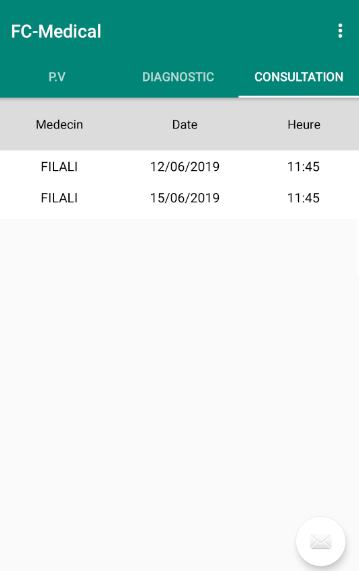
\includegraphics[width=7cm,height=7cm,keepaspectratio]{Application/dossier5.png}
% \caption{ Interface de Consultation}
% \end{figure}

% Contient les Rendez-vous que le patient a avec un médecin
% \subsection{Interface de Traitement }
% \begin{figure}[H]
%   \centering
% 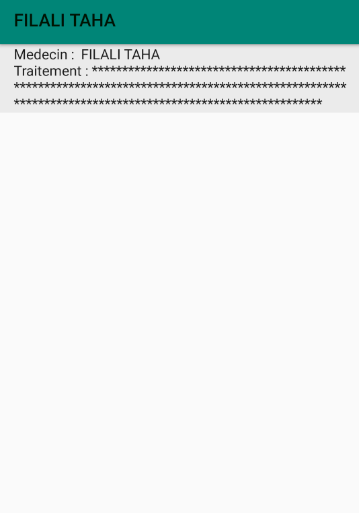
\includegraphics[width=7cm,height=7cm,keepaspectratio]{Application/trait1.png} 
% \caption{ Interface de Traitement}
% \end{figure}

% Cette interface contient les mesures appliquées par le médecin au patient afin de l'aider à en guérir, de soulager ses symptômes, ou encore d'en prévenir l'apparition.

% Si Le patient n'a pas un dossier médicale une boite dialog s'affiche pour demender au patient s'il vaut creér un maintenant ou non.
% \begin{figure}[H]
%   \centering
% 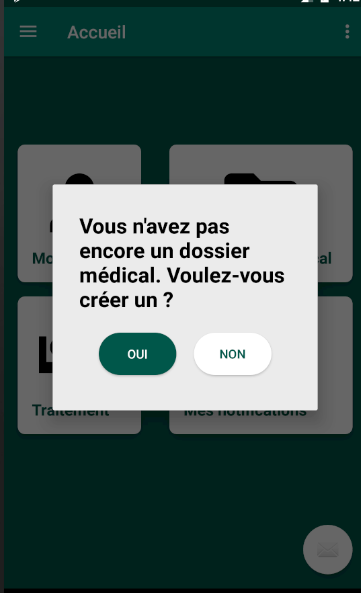
\includegraphics[width=8cm,height=8cm,keepaspectratio]{Application/dossier8.png} 
% \caption{ Interface de demender de creation un dossier médicale}
% \end{figure}

% \newpage
% \section{Les interfaces du medécin }
% \subsection{Interface d'accueil }
% \begin{figure}[H]
%   \centering
% 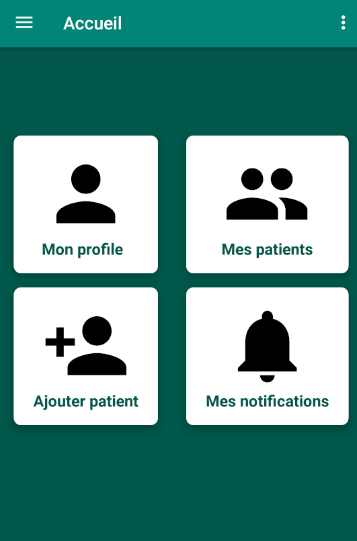
\includegraphics[width=7cm,height=7cm,keepaspectratio]{Application/medecin1.png} 
% \caption{ Interface de d'acceuil du medécin}
% \end{figure}

% Cette figure ci-dessus montre la page d’accueil qui va apparaitre dès qu’un médecin lance l’application après s'authentification  . Cet interface comporte un GridView contient  4 figures sont  "Mon Profil" ,"Mes patients","Ajouter patient" et "Mes Notification" , qui en cliquant sur une figure , va nous diriger vers L'interface que nous avons choisie  .
% rface d’accueil du patient

% \subsection{Interface de patients de medécin }
% \begin{figure}[H]
%   \centering
% 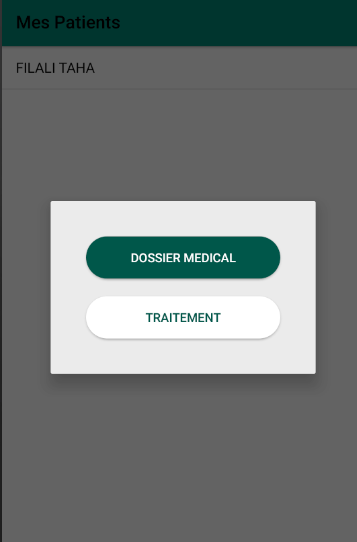
\includegraphics[width=7cm,height=7cm,keepaspectratio]{Application/mespatient1.png}
% \caption{ Interface de patients de medécin}
% \end{figure}


% En cette interface on aura une liste des patients que le médecin suive.
% En cliquant sur un élément,une boite de dialogue s'affichera et nous demande de choiser si aller vers le dossier medical du patient pour le consulter ou le modifier,si aller vers l'interface du traitement ou le médecin peut saisir le traitement que le patient doit suivre.


% \subsection{Interface d'ajouter un patient}
% \begin{figure}[H]
%   \centering
% 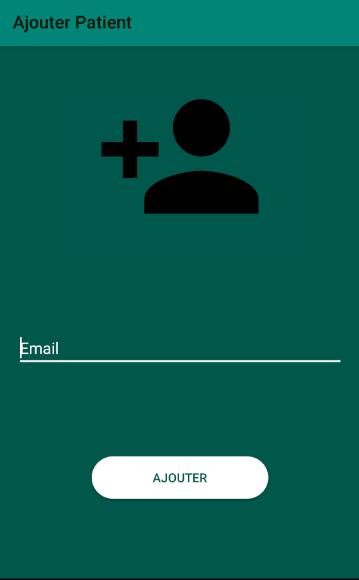
\includegraphics[width=7cm,height=7cm,keepaspectratio]{Application/ajo2.png} 
% \caption{Interface d'ajouter un patient}
% \end{figure}

% Dans cette interface le médecin peut envoyer une invitation par saisir l'email du patient requis.


\section*{conclusion }
Ce chapitre décrit les interfaces graphique du l'application et ses fonctionnements qui sont utilisés par l'utilisateur . 